% based on https://vtex-soft.github.io/texsupport.isba-ba/
% \documentclass[ba,preprint]{imsart}% use this for supplement article
\documentclass[]{imsart}

\pubyear{\the\year{}}
\volume{TBA}
\issue{TBA}
\doi{999999999/chaine\_aléatoire/test}

\firstpage{1}
\lastpage{1}

%
\usepackage{amsthm}
\usepackage{amsmath}
\usepackage{natbib}
\usepackage[colorlinks,citecolor=blue,urlcolor=blue,filecolor=blue,backref=page]{hyperref}
\usepackage{graphicx}

\startlocaldefs
\numberwithin{equation}{section}
\theoremstyle{plain}
\newtheorem{thm}{Theorem}[section]
\endlocaldefs
% rticles required

% tightlist command for lists without linebreak
\providecommand{\tightlist}{%
  \setlength{\itemsep}{0pt}\setlength{\parskip}{0pt}}

% From pandoc table feature
\usepackage{longtable,booktabs,array}
\usepackage{calc} % for calculating minipage widths
% Correct order of tables after \paragraph or \subparagraph
\usepackage{etoolbox}
\makeatletter
\patchcmd\longtable{\par}{\if@noskipsec\mbox{}\fi\par}{}{}
\makeatother
% Allow footnotes in longtable head/foot
\IfFileExists{footnotehyper.sty}{\usepackage{footnotehyper}}{\usepackage{footnote}}
\makesavenoteenv{longtable}


% Pandoc header

\begin{document}
\begin{frontmatter}

\title{Analyse Exploratoire des Données clients d'un opérateur télécom}
\runtitle{Analyse Exploratoire des Données clients d'un opérateur télécom}

\begin{aug}
\author{Mehdi Mansour\thanksref{addr1}\ead[label=ea-1,email]{mehdi.mansour@univ-lyon2.fr}}
\runauthor{Mansour}

 %loop through affiliations
\address[addr1]{L3\_Data\_Science, ICOM, 5 Av. Pierre Mendès France, 69500 Bron \ifstrequal{addr1}{addr1}{\printead{ea-1}}{}
%authors
}%affiliations


\end{aug}

\begin{abstract}
Dans ce travail, le set de données contient des informations sur les clients d'une entreprise de télécommunications. Il comprend 100 variables pour chaque client, telles que leur âge, leur lieu de résidence, leur historique d'utilisation de services téléphoniques et leur comportement de paiement. L'objectif étant de mettre en application les techniques d'analyse exploratoire et de réduction d dimension
Le choix de ce jeu est un compromis répondant à plusieurs besoins. D'abord l'analyse de ce type de données est un réel enjeu économique en entreprise. Ensuite, le volume et le nombre de variables offrent un réel défi technique pour les méthodes vues en cours. Également, et en articulant ce module avec le module de statistiques inférentielles et de modélisation linéaire, ce jeu est propice à la résolution d'autres problématiques que je compte mettre en œuvre cet été.
\end{abstract}

% MSC class

% keywords
 \begin{keyword} \kwd{PCA} \kwd{AFC} \kwd{ACM} \kwd{T-SNE} \kwd{Inférence} \kwd{Prédiction}\end{keyword}
\end{frontmatter}

\hypertarget{introduction}{%
\section{Introduction}\label{introduction}}

~

~~~Les entreprises collectent une quantité considérable de données sur leurs clients, allant des informations de base telles que les noms et les adresses, aux habitudes d'achat, aux préférences personnelles et aux données comportementales en ligne. Les données d'utilisation des clients constituent un atout précieux pour les entreprises, car elles permettent de comprendre les préférences et les besoins de leurs clients, ce qui leur permet de personnaliser leur offre et d'améliorer leur expérience client. En outre, ces données peuvent également être utilisées pour anticiper les tendances du marché et pour prendre des décisions commerciales éclairées.

~

Ces données, par leur volume et le nombre de variables considérable, deviennent vite illisibles/inexploitables, sans des méthodes adaptées pour en extraire la précieuse information. Les techniques de réduction de dimensions abordées dans notre module, font partie de notre arsenal de futurs professionnels de la data. Nous allons essayer de les appliquer à un jeu de données d'un fournisseur d'accès internet-mobile. Ce jeu de données contient initialement 100k observations, pour un total d'une centaine de variables. Nous allons pas à pas essayer de le comprendre, le traiter, et interpréter les précieuses informations qu'il recèle.

~

\hypertarget{pruxe9sentation-du-jeu-de-donnuxe9es}{%
\section{Présentation du jeu de données}\label{pruxe9sentation-du-jeu-de-donnuxe9es}}

~

~~~Il s'agit d'un ensemble de données contenant des informations sur les habitudes de consommation des clients d'une entreprise de télécommunications. Il y a un total de 100 000 observations (lignes) et 100 variables (colonnes). Les variables sont de types différents (float, integer, character) et sont présentées sous forme de colonnes avec des noms tels que ``rev\_Mean'', ``mou\_Mean'', ``totmrc\_Mean'', etc. Les valeurs dans chaque colonne indiquent des moyennes, des totaux ou des moyennes sur des périodes spécifiques. Certaines variables concernent des informations personnelles des clients, telles que leur âge, leur revenu ou leur statut familial, tandis que d'autres variables concernent les données relatives à leur utilisation des services de télécommunications.

~

Voici l'entête du set de données, dont nous allons étayer les premières colonnes dans la suite:

~

~

\begin{verbatim}
##   rev_Mean mou_Mean totmrc_Mean da_Mean ovrmou_Mean ovrrev_Mean vceovr_Mean
## 1  23.9975   219.25      22.500  0.2475        0.00         0.0         0.0
## 2  57.4925   482.75      37.425  0.2475       22.75         9.1         9.1
## 3  16.9900    10.25      16.990  0.0000        0.00         0.0         0.0
## 4  38.0000     7.50      38.000  0.0000        0.00         0.0         0.0
## 5  55.2300   570.50      71.980  0.0000        0.00         0.0         0.0
## 6  82.2750  1312.25      75.000  1.2375        0.00         0.0         0.0
\end{verbatim}

~

Dans ce jeu, les observations sont numérotées de 1 à 100 000, chaque observation va contenir 100 attributs, dont des données quantitatives comme :

~

\textbf{rev\_Mean} : Revenu mensuel moyen (montant facturé).

\textbf{mou\_Mean} : Nombre moyen de minutes d'utilisation mensuelle.

\textbf{totmrc\_Mean} : Charge mensuelle moyenne totale récurrente.

\textbf{da\_Mean} : Nombre moyen d'appels assistés par annuaire.

\textbf{ovrmou\_Mean} : Minutes moyennes d'utilisation supplémentaires.

\textbf{ovrrev\_Mean} : Revenu moyen supplémentaire.

\textbf{vceovr\_Mean} : Revenu moyen de dépassement de minutes d'appel.

~

Ainsi que des données catégorielles telles que :

~

\textbf{marital} : Statut matrimonial

\textbf{ownrent}: Statut de propriétaire ou locataire.

\textbf{dwlltype}: Type d'unité de logement.

\textbf{ethnic}: Code de regroupement ethnique.

~

Voici la liste complète des variables:

~

`months', `uniqsubs', `actvsubs', `totcalls', `adjqty', `avg3mou', `avg3qty', `avg3rev', `rev\_Mean', `mou\_Mean', `totmrc\_Mean', `da\_Mean', `ovrmou\_Mean', `ovrrev\_Mean', `vceovr\_Mean', `datovr\_Mean', `roam\_Mean', `change\_mou', `change\_rev', `drop\_vce\_Mean', `drop\_dat\_Mean', `blck\_vce\_Mean', `blck\_dat\_Mean', `unan\_vce\_Mean', `unan\_dat\_Mean', `plcd\_vce\_Mean', `plcd\_dat\_Mean', `recv\_vce\_Mean', `recv\_sms\_Mean', `comp\_vce\_Mean', `comp\_dat\_Mean', `custcare\_Mean', `ccrndmou\_Mean', `cc\_mou\_Mean', `inonemin\_Mean', `threeway\_Mean', `mou\_cvce\_Mean', `mou\_cdat\_Mean', `mou\_rvce\_Mean', `owylis\_vce\_Mean', `mouowylisv\_Mean', `iwylis\_vce\_Mean', `mouiwylisv\_Mean', `peak\_vce\_Mean', `peak\_dat\_Mean', `mou\_peav\_Mean', `mou\_pead\_Mean', `opk\_vce\_Mean', `opk\_dat\_Mean', `mou\_opkv\_Mean', `mou\_opkd\_Mean', `drop\_blk\_Mean', `attempt\_Mean', `complete\_Mean', `callfwdv\_Mean', `callwait\_Mean', `totmou', `totrev', `adjrev', `adjmou', `avgrev', `avgmou', `avgqty', `avg6mou', `avg6qty', `avg6rev', `hnd\_price', `phones', `models', `truck', `rv', `lor', `adults', `income', `numbcars', `forgntvl', `eqpdays', `churn', `new\_cell', `crclscod', `asl\_flag', `prizm\_social\_one', `area', `dualband', `refurb\_new', `hnd\_webcap', `ownrent', `dwlltype', `marital', `infobase', `HHstatin', `dwllsize', `ethnic', `kid0\_2', `kid3\_5', `kid6\_10', `kid11\_15', `kid16\_17', `creditcd'.

~

Elles sont répertoriées avec leurs significations respectives en \textbf{Annexe I}.

~

~

\hypertarget{pruxe9traitement-des-donnuxe9es-nettoyage-recodage-et-pruxe9paration-pour-lanalyse}{%
\section{Prétraitement des données : nettoyage, recodage et préparation pour l'analyse}\label{pruxe9traitement-des-donnuxe9es-nettoyage-recodage-et-pruxe9paration-pour-lanalyse}}

~

\hypertarget{identification-des-colonnes-napportant-pas-dinformation-utile-uxe0-lanalyse}{%
\subsection{Identification des colonnes n'apportant pas d'information utile à l'analyse:}\label{identification-des-colonnes-napportant-pas-dinformation-utile-uxe0-lanalyse}}

~

Dans notre jeu, il s'agit de la colonne `Customer\_Id' , qui attribue un numéro client à chaque usager. Bien qu'elle l'identifie de façon unique, cette valeur est extrinsèque au sujet. Dans le sens ou elle n'apporte pas d'information pertinente sur les caractéristiques ou le comportement de l'individu qu'elle identifie. Cette colonne est cépendant utile pour faire des jointures avec d'autres tables de données.

~

\hypertarget{identification-des-colonnes-inexploitables-par-manque-de-valeurs}{%
\subsection{Identification des Colonnes inexploitables par manque de valeurs:}\label{identification-des-colonnes-inexploitables-par-manque-de-valeurs}}

~

Dans notre set de données initial, il existe des valeurs manquantes identifiées et portant la mention ``n.a'' (not available).D'après la littérature, le seuil acceptable de données manquantes peut dépendre de plusieurs facteurs tels que le type de données, la taille de l'échantillon, la méthode d'analyse et le domaine d'application. Certains chercheurs ont suggéré des seuils spécifiques pour différents types de données. Par exemple un seuil de 5\% pour les données catégorielles et un seuil de 10\% pour les données continues. Dans cette phase, nous retiendrons ( choix de travail) un seuil éliminatoire exigeant de 5\% pour les deux types de données.

~

Le code suivant suivant permet d'identifier les colonnes avec moins de 95\% de valeurs disponibles, et de les écarter de notre dataset en cours de ``preprocessing''.

~

\begin{verbatim}
# Définition d'un seuil de tolérance

seuil.acceptable = 0.05

# Identification de colonnes concernées et affichage de leurs noms

proportion.valeurs.manquantes = colSums(is.na(d))/nrow(d)

colonnes.peu.remplies = 
names(proportion.valeurs.manquantes[proportion.valeurs.manquantes > seuil.acceptable])

colonnes.peu.remplies
\end{verbatim}

\begin{verbatim}
## [1] "hnd_webcap" "lor"        "adults"     "income"     "numbcars"
\end{verbatim}

\begin{verbatim}
# Ecartement des colonnes identifiées "pauvres" du Dataset 

d.travail = subset(d, select = -c(hnd_webcap, lor, adults, income, numbcars))
\end{verbatim}

~

Avec un seuil aussi exigeant, notre dataset initial est suffisamment de qualité pour n'avoir que 5 variables concernées. La variable ``income'' aurait pu être problématique à supprimer car le revenu d'un consommateur est une donnée cruciale dans un rapport commercial. Néanmoins, nous nous rendons compte que cette variable le ``revenu estimé'' et non ``réel'' du client. C'est à dire que la variable ``income'' est une synthèse d'autres variables disponibles sur le client, soit une raison supplémentaire de l'écarter de la phase d'analyse du moins.

~

Nous travaillerons désormais avec le dataset d.travail, épuré de cinq variables, et que nous allons affiner dans le but d'optimiser nos résultats d'analyse.

~

\hypertarget{recoder-des-modalituxe9s}{%
\subsection{Recoder des modalités:}\label{recoder-des-modalituxe9s}}

~

Dans le dataset, plusieurs variables catégorielles ont une modalité chaine vide ````, il n'y a pas d'information permettant de savoir s'il s'agit de données indisponibles, non saisies, ou non exprimées par le client. Nous nous contenterons pour l'instant de leur attribuer la nomenclature''inconnue'', grâce au code suivant:

\begin{verbatim}
# Boucle sur chaque colonne pour remplacer la valeur "" en "inconnue":
for ( colonne in colnames(d.travail)){
  d.travail[,colonne] = ifelse(d.travail[,colonne] == "", "inconnue", d.travail[,colonne])
}
\end{verbatim}

~

\hypertarget{choisir-une-population-repruxe9sentative-ruxe9duite}{%
\subsection{Choisir une population représentative réduite:}\label{choisir-une-population-repruxe9sentative-ruxe9duite}}

~

Suite à des essais de requêtes sur le dataset initial, le projet ambitieux de travailler sur les 10M de cases disponibles, s'est vite confronté aux limites de mémoire et de puissance de calcul sur mon terminal. D'ou la nécessité de choisir une méthode pour réduire le volume de données à prendre en considération dans l'analyse, sans dégrader la pertinence des resultats obtenus.

~

La méthode probabiliste de l'échantillonnage aléatoire simple est retenue, avec un ratio de réduction de 1/20 :

~

Sur les 100k lignes disponibles, 5000 lignes sont successivement choisies au hasard, sans remise.

~

\begin{verbatim}
# Confection d'un échantillon représentatif des observations:

set.seed(123)  # pour la reproductibilité si chunk rejouée

echantillon.travail = d.travail[sample(nrow(d.travail), 5000, replace = FALSE), ]
\end{verbatim}

~

La comparaison de statistiques descriptives telles que la moyenne, médiane et les quartiles des variables de l'échantillon versus le set complet, donne une idée sur leurs distributions respectives, et permet de détecter des anomalies potentielles d'échantillonnnage.

~

Exemple, pour la variable \textbf{mou\_Mean} nous obtenons le graphique boxplot suivant:

~

\begin{flushleft}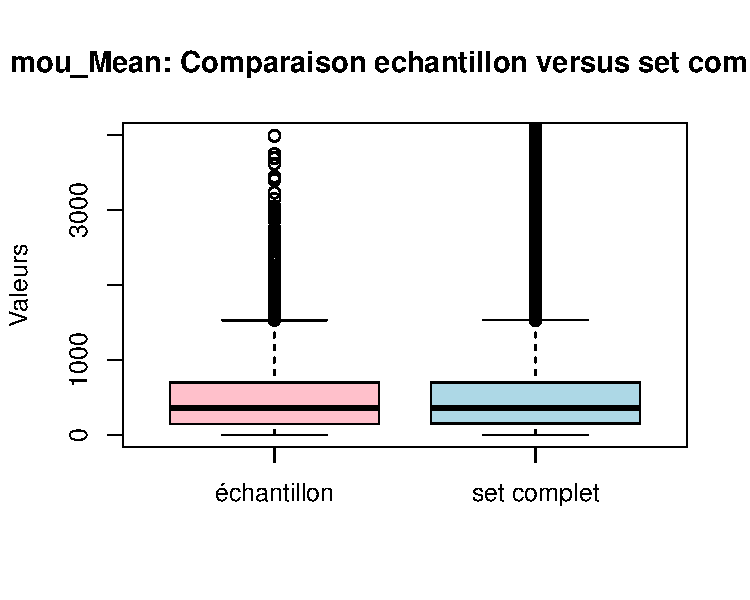
\includegraphics{Analyse_Exploratoire_Projet_files/figure-latex/unnamed-chunk-8-1} \end{flushleft}

~

Pour la variable \textbf{rev\_Mean} nous obtenons le graphique boxplot suivant:

~

\begin{flushleft}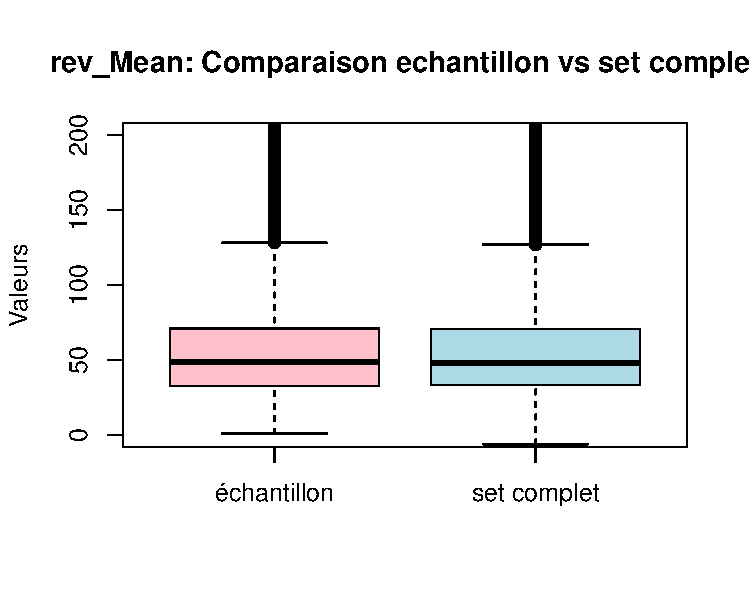
\includegraphics{Analyse_Exploratoire_Projet_files/figure-latex/unnamed-chunk-9-1} \end{flushleft}

~

La similarité de la distribution des variables entre l'échantillon et le set complet, permet de nous rassurer sur le caractère représentatif du sous-ensemble choisi. Un tirage aléatoire qui se serait mal executé nous aurait alerté par une modification significative des statistiques telles que la moyenne, la médiane et les quartiles.

~

\hypertarget{analyse-des-donnuxe9es-quantitatives}{%
\section{Analyse des données quantitatives}\label{analyse-des-donnuxe9es-quantitatives}}

~

\hypertarget{probluxe9matique}{%
\subsection{Problématique:}\label{probluxe9matique}}

~

Suite au travail préliminaire d'exploration, d'élimination, et à l'échantillonnage, nous disposons à ce stade d'un set de 5000 observations représentatives et de de 95 variables.

~

Nous pouvons légitimement exclure \textbf{churn} de l'analyse quantitative, car cette variable prend des valeurs numériques de 0 ou 1, mais exprime en réalité les modalité résilié ou non-résilié d'un abonnement.

~

La variable \textbf{Customer\_ID} est également inutile pour l'analyse car elle sert juste d'attribut d'identification.

~

Les variables quantitatives restantes sont au nombre de 73 ce qui est un nombre élevé, pouvant rendre coûteuse en temps et en ressources la transformation de ces données en décisions ou actions commerciales.

~

Par exemple, sur un terminal avec un processeur i5 de 8ème génération et 16 gb de ram, la tentative de réaliser une régression logistique permettant de prédire la résiliation d'un abonnement avec ces 73 variables, s'est soldée par un échec: l'ordinateur rame et finit par bugger.

~

Cela nous amène à la nécéssité de synthétiser l'information contenue ce dataset dans moins de variables : réduire la dimension du dataset tout en gardant un maximum d'information.

~

Observons la nature du lien entre variables dans cette matrice de corrélation linéaire entre variables centrées et réduites:

~

\begin{verbatim}
# Construisons un set de données centrées réduites:

moyennes = apply(e.t.quant, 2, mean, na.rm=TRUE)

ecarts_types_biaisés = apply(e.t.quant, 2, sd, na.rm=TRUE) * (sqrt(4999/5000))

centree = sweep(e.t.quant, 2, moyennes, "-")

centree_reduite = sweep(centree, 2, ecarts_types_biaisés, "/")

cor = cor(centree_reduite, use="complete.obs")

corrplot(cor, method = "circle")
\end{verbatim}

\begin{flushleft}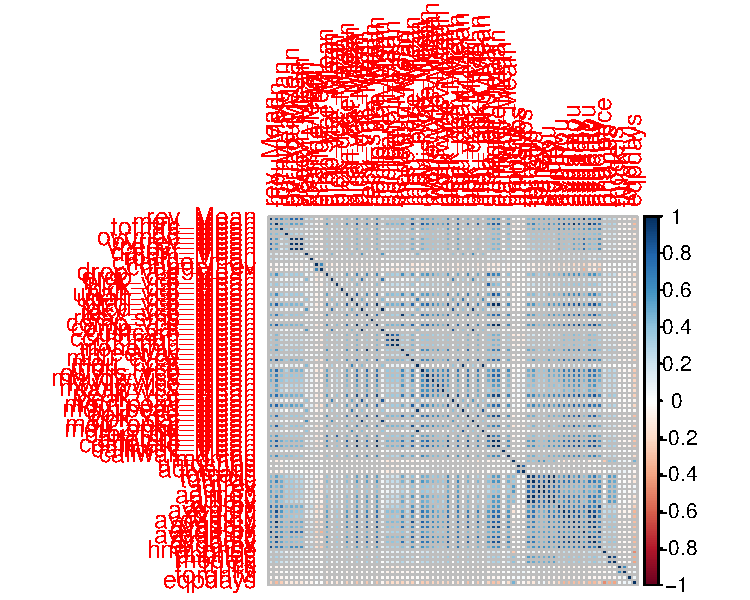
\includegraphics{Analyse_Exploratoire_Projet_files/figure-latex/unnamed-chunk-11-1} \end{flushleft}

~

L'observation des coefficients de corrélation linéaire entre les différentes variables montre des liens \textbf{linéaires} et majoritairement positifs entre beaucoup de variables. Ces variables linéairement corrélées peuvent apriori être synthétisées en variables composites moins nombreuses. C'est ce que nous allons essayer de faire avec la \textbf{PCA}, analyse en composantes principales.

~

\hypertarget{application-dune-analyse-en-composantes-principales-aux-donnuxe9es-quantitatives}{%
\subsection{Application d'une analyse en composantes principales aux données quantitatives:}\label{application-dune-analyse-en-composantes-principales-aux-donnuxe9es-quantitatives}}

~

Nous utiliserons dans la suite, les outils mis à disposition par la librairie FActoMineR.

~

\hypertarget{imputation-et-ruxe9alisation-de-la-pca}{%
\subsubsection{Imputation et réalisation de la PCA:}\label{imputation-et-ruxe9alisation-de-la-pca}}

~

Malgré une élimination d'emblée des variables mal renseignées, nos variables gardent entre 0 et 5\% des valeurs qui ne sont pas remplies. Pour optimiser la PCA, il est nécéssaire de les \textbf{imputer}, c'est à dire les compléter avec une méthode optimisant la précision du résultat. Dans ce cas, nous excluons les imputations par la moyenne ou la médiane, qui réduisent la variance et induisent des biais. Au profit d'une imputation qui tient compte de la structure des données existantes.

~

Voici les lignes de code permettant l'imputation et la réalisation de la PCA

~

\begin{verbatim}
# Estimer le nombre de dimensions principales nécessaires à une bonne complétion des données manquantes

resultat.estimation = estim_ncpPCA(e.t.quant, ncp.max=10) 

# Imputation

resultat.completion = imputePCA(e.t.quant, ncp=resultat.estimation$ncp) 

# Réaliser la PCA normée sur le set de données complétées

resultat.pca = PCA(resultat.completion$completeObs, scale.unit=TRUE, ncp = 10, graph = FALSE) 
\end{verbatim}

~

\hypertarget{choix-du-nombre-daxes-uxe0-retenir}{%
\subsubsection{Choix du nombre d'axes à retenir:}\label{choix-du-nombre-daxes-uxe0-retenir}}

~

Observons les valeurs propres de chaque axe factoriel afin de déterminer ceux à retenir:

~

\begin{flushleft}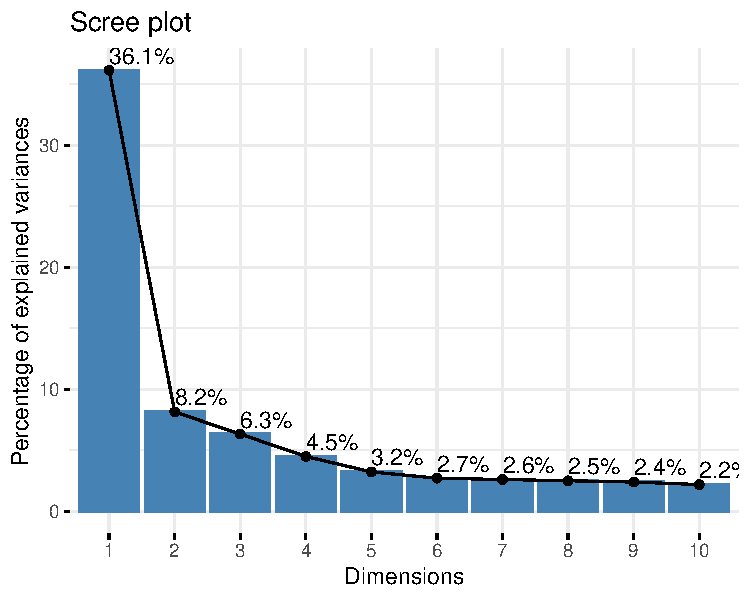
\includegraphics{Analyse_Exploratoire_Projet_files/figure-latex/unnamed-chunk-13-1} \end{flushleft}

~

Le premier axe capture une grande partie de la variance de donnée, le critère du coude permet de retenir le deuxième axe également. Le critère de Kaiser retient également le deuxième axe.

~

Conclusion : nous retenons le premier et le deuxième axe ce qui permettera de capturer 44.3\% de la variance de nos données initiales.

~

\hypertarget{interpruxe9tation-des-variables}{%
\subsubsection{Interprétation des Variables:}\label{interpruxe9tation-des-variables}}

~

~

Apprécions la contribution et le cos2 des variables dans le plan factoriel choisi:

~

\begin{flushleft}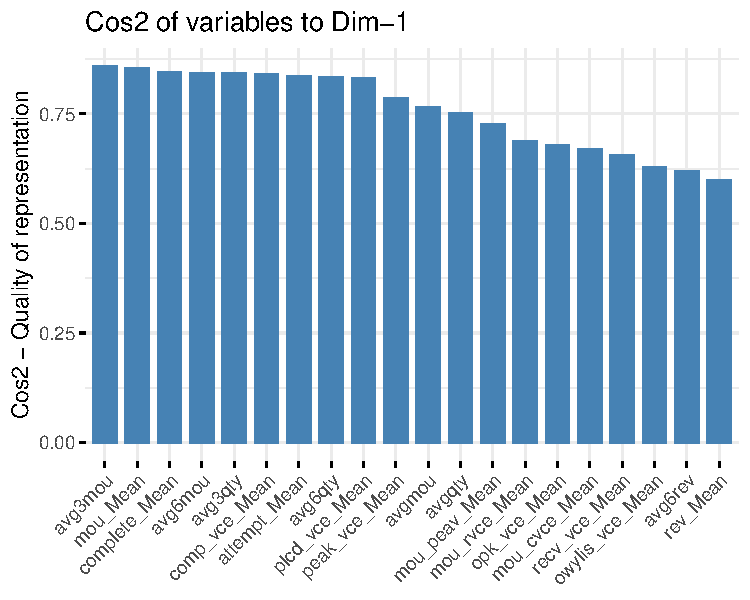
\includegraphics{Analyse_Exploratoire_Projet_files/figure-latex/unnamed-chunk-15-1} \end{flushleft}

\begin{flushleft}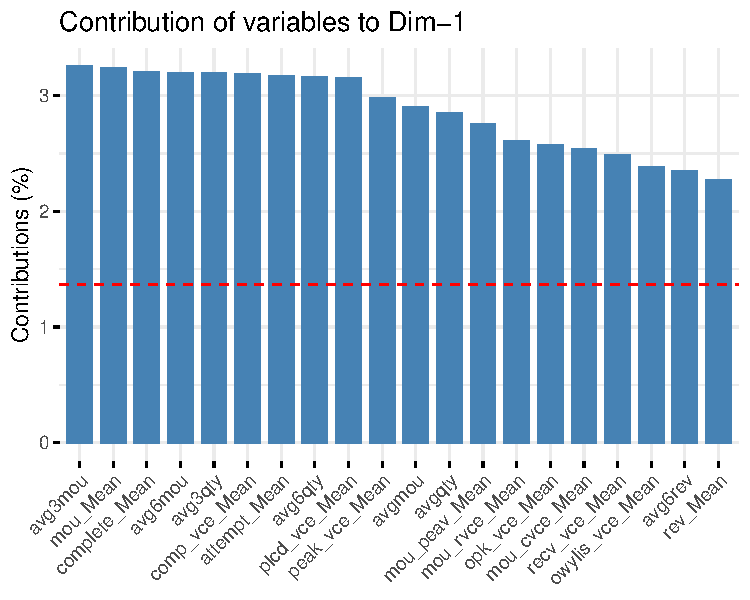
\includegraphics{Analyse_Exploratoire_Projet_files/figure-latex/unnamed-chunk-15-2} \end{flushleft}

\begin{flushleft}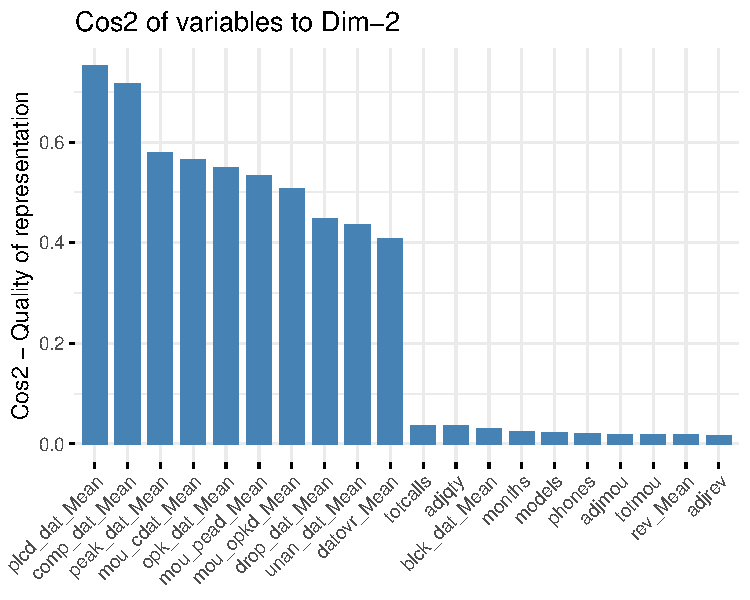
\includegraphics{Analyse_Exploratoire_Projet_files/figure-latex/unnamed-chunk-15-3} \end{flushleft}

\begin{flushleft}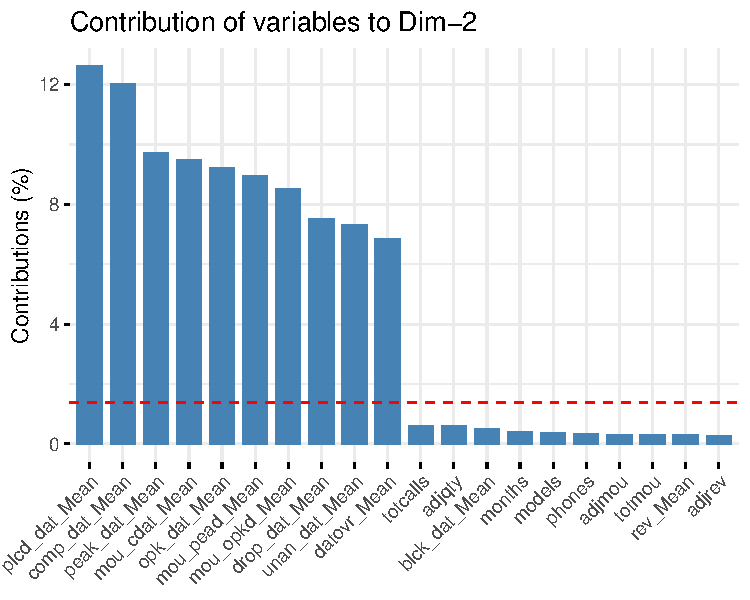
\includegraphics{Analyse_Exploratoire_Projet_files/figure-latex/unnamed-chunk-15-4} \end{flushleft}

~

Projetons les variables qui contribuent le plus au plan factoriel:

~

\begin{flushleft}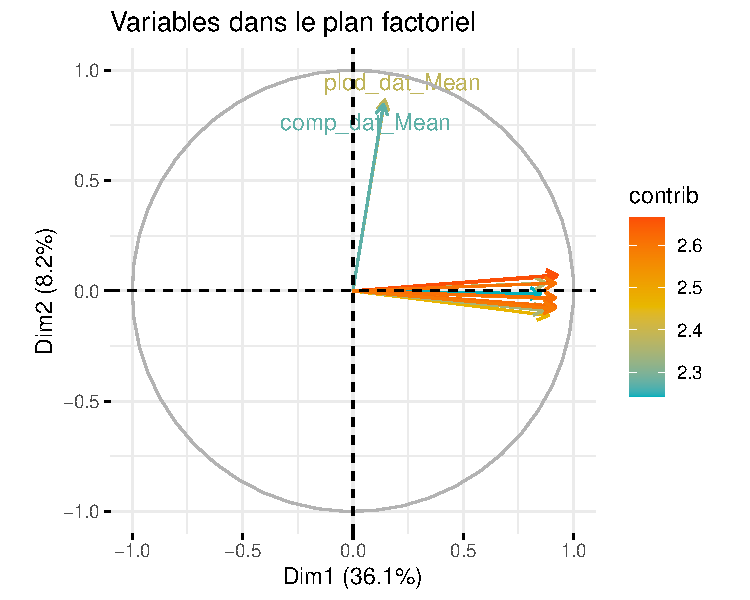
\includegraphics{Analyse_Exploratoire_Projet_files/figure-latex/unnamed-chunk-16-1} \end{flushleft}

~

**Sémantique des variables:

~

(L'annexe 1 donne la signification exacte de la nomenclature chaque variable.)

~

les variables ``avg3mou'', ``mou\_Mean'', ``complete\_Mean'', ``avg6mou'', ``avg\_qty'', ``comp\_vce\_Mean'', ``attemp\_Mean'', ``avg6qty'', ``plcd\_vce\_Mean'' caractérisent le côté positif du premier axe factoriel, les individus qui seront projetés du côté positif de l'axe 1 auront des valeurs élevées sur ces variables. C'est à dire, des individus qui passent un nombre élevé d'appels, et qui auront une durée longue de leurs communications.

~

les variables ``plcd\_dat\_Mean'', ``comp\_dat\_Mean'' caractérisent le côté positif du deuxième axe factoriel, les individus qui seront projetés du côté positif de l'axe 2 auront des valeurs élevées sur ces variables. C'est à dire , des individus qui tentent, en réussissant ou pas, d'utiliser l'internet du mobile.

~

La PCA actuelle ne permet pas de caractériser significativement les côtés négatifs de ces deux axes. Ceci est certainement un indicateur d'une performance non optimale sur ce dataset.

~

\hypertarget{interpruxe9tation-des-individus}{%
\subsubsection{Interprétation des individus:}\label{interpruxe9tation-des-individus}}

~

Apprécions la contribution et le cos2 des individus dans le plan factoriel choisi :

~

\begin{flushleft}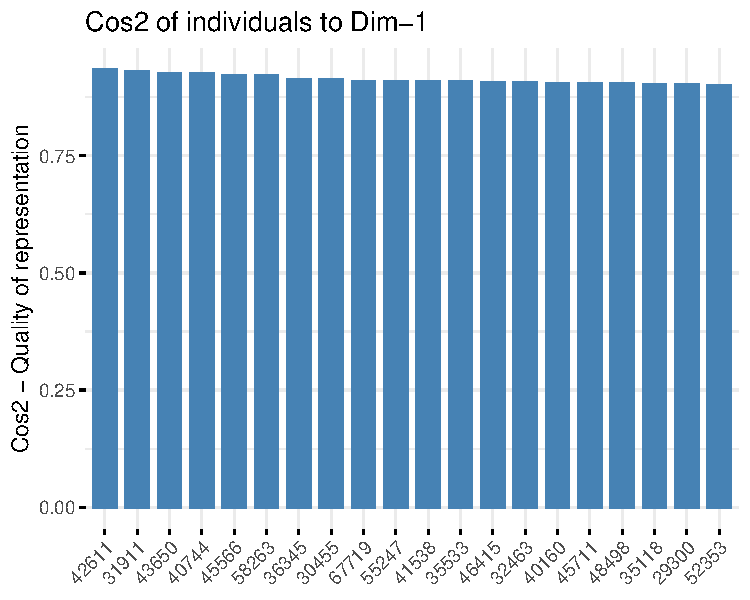
\includegraphics{Analyse_Exploratoire_Projet_files/figure-latex/unnamed-chunk-18-1} \end{flushleft}

\begin{flushleft}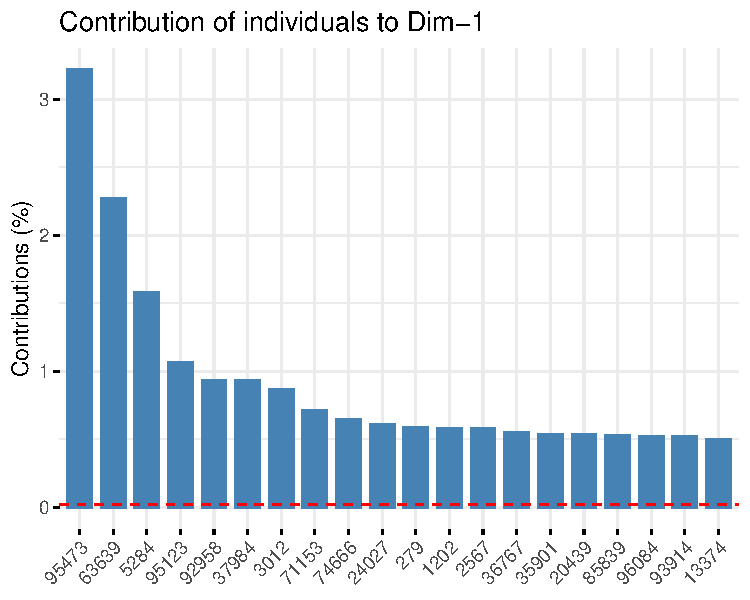
\includegraphics{Analyse_Exploratoire_Projet_files/figure-latex/unnamed-chunk-18-2} \end{flushleft}

\begin{flushleft}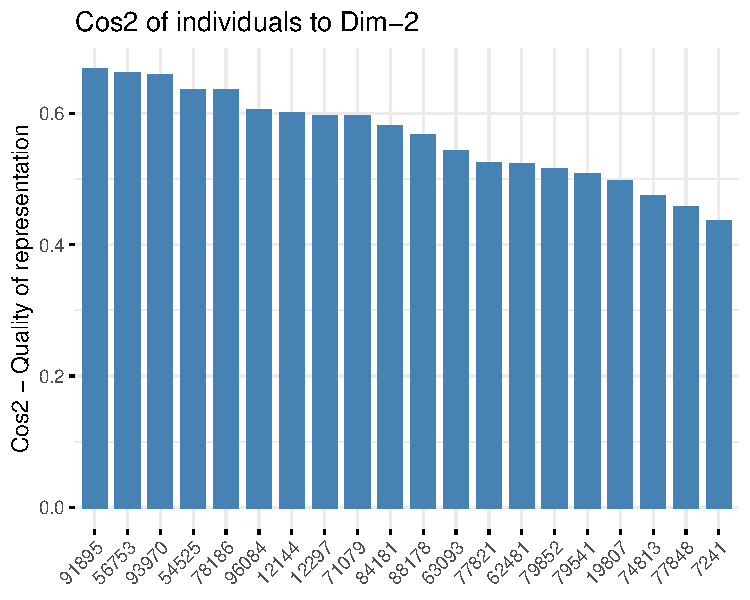
\includegraphics{Analyse_Exploratoire_Projet_files/figure-latex/unnamed-chunk-18-3} \end{flushleft}

\begin{flushleft}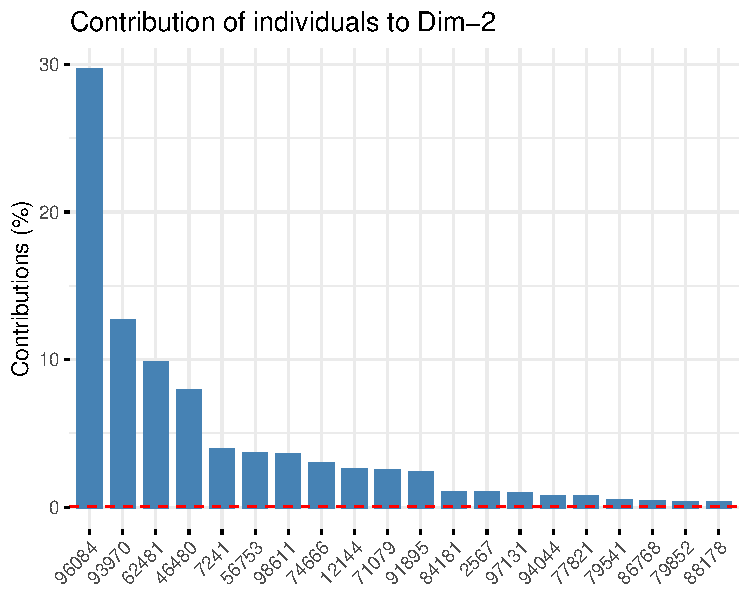
\includegraphics{Analyse_Exploratoire_Projet_files/figure-latex/unnamed-chunk-18-4} \end{flushleft}

~

Projetons les individus qui contribuent le plus au plan factoriel:

~

\begin{flushleft}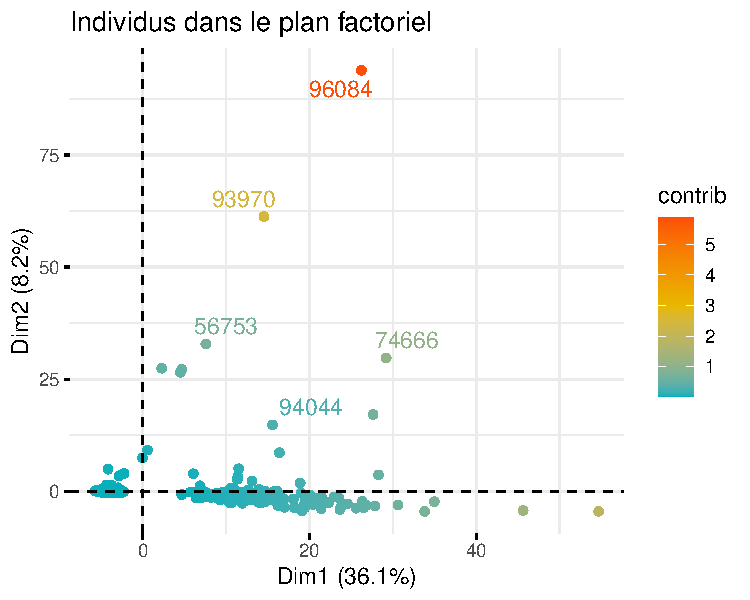
\includegraphics{Analyse_Exploratoire_Projet_files/figure-latex/unnamed-chunk-19-1} \end{flushleft}

**Sémantique des individus:

~

Des individus comme ``40136'', ``21377'', ``46129'', ``88317'' et ``23331'' caractérisent le côté positif du premier axe factoriel, ces individus ont des valeurs élevées en ``avg3mou'', ``mou\_Mean'', ``complete\_Mean'', ``avg6mou'', ``avg\_qty'', ``comp\_vce\_Mean'', ``attemp\_Mean'', ``avg6qty'' et ``plcd\_vce\_Mean''.

~

Des individus comme ``96084'', ``93970'', ``56753'', ``12144'' caractérisent le côté positif du deuxième axe factoriel, ces individus ont des valeurs élevées en ``plcd\_dat\_Mean'' et ``comp\_dat\_Mean''.

~

Des individus comme ``42611'', ``31911'', ``43650'' et ``40744'' sont bien projetés du coté négatif du premier axe factoriel mais sans avoir suffisamment de contribution pour pouvoir le caractériser.

~

\textbf{Observation générale} : il est à remarquer que suite à ce premier essai de reduction de dimensionnalité, la projection des individus dans le plan factoriel laisse apparaitre des zones de nuage d'observations denses et bien projetées. Nous pouvons émettre l'hypothèse qu'ils s'agisse d'individus à profil similaire. Dans la suite, la technique T-sne sera utilisée pour essayer de confirmer cette hypothèse.

~

\hypertarget{mise-en-pratique-de-t-sne-pour-visualiser-des-similarituxe9s-entre-observations}{%
\subsection{Mise en pratique de T-SNE, pour visualiser des similarités entre observations:}\label{mise-en-pratique-de-t-sne-pour-visualiser-des-similarituxe9s-entre-observations}}

~

Ce qui suit, répond à une problématique du type : visualiser la proximité entre individus dans un espace réduit, détecter potentiellement des clusters (de profil de consommation par exemple).

~

L'algorithme T-sne est appliqué aux données centrées réduites, successivement, en jouant sur les hyper-paramètres : perplexité, pas d'apprentissage (learning rate) et nombre maximal d'itérations.

~

Nous obtenons respectivement les graphiques suivants:

~

\begin{flushleft}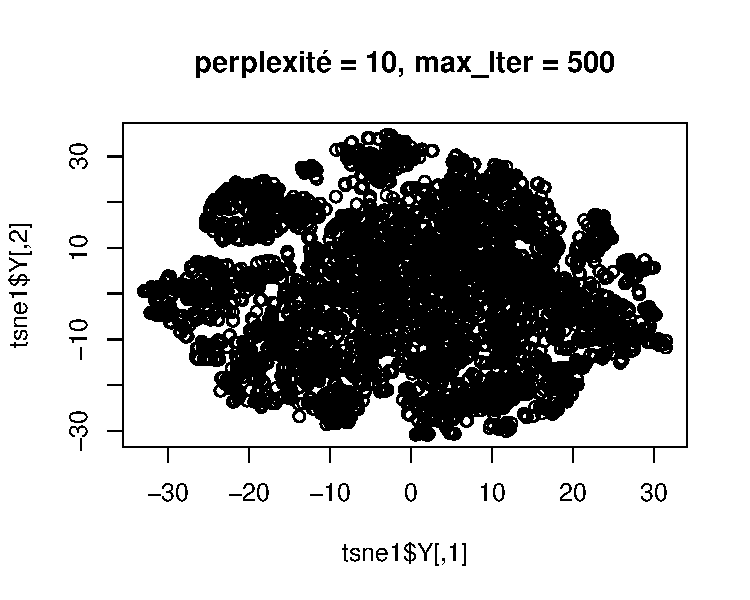
\includegraphics{Analyse_Exploratoire_Projet_files/figure-latex/unnamed-chunk-20-1} \end{flushleft}

\begin{flushleft}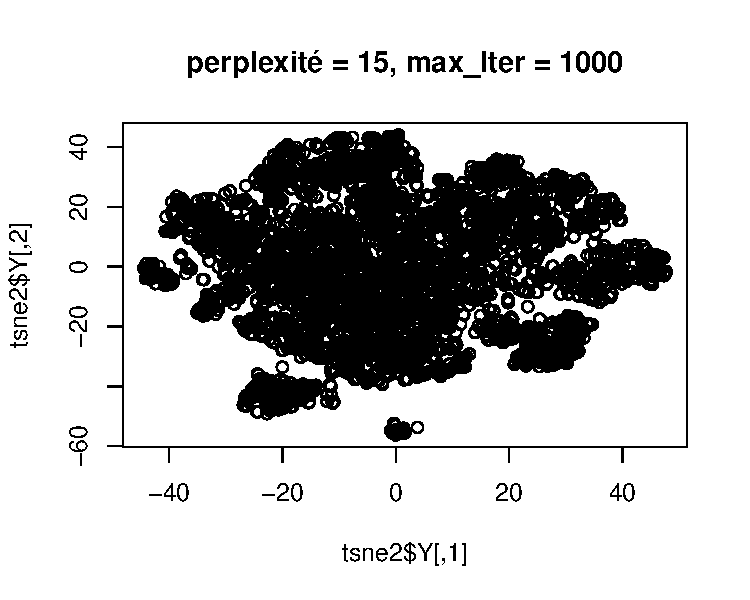
\includegraphics{Analyse_Exploratoire_Projet_files/figure-latex/unnamed-chunk-20-2} \end{flushleft}

\begin{flushleft}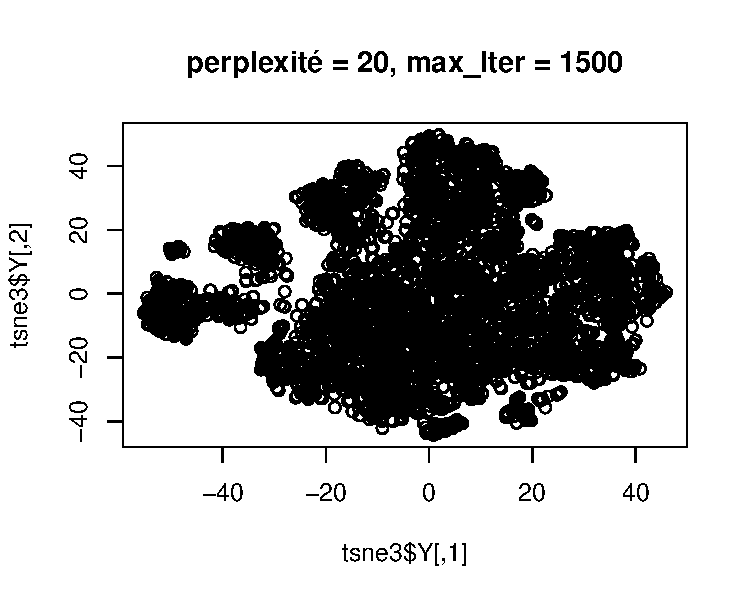
\includegraphics{Analyse_Exploratoire_Projet_files/figure-latex/unnamed-chunk-20-3} \end{flushleft}

\begin{flushleft}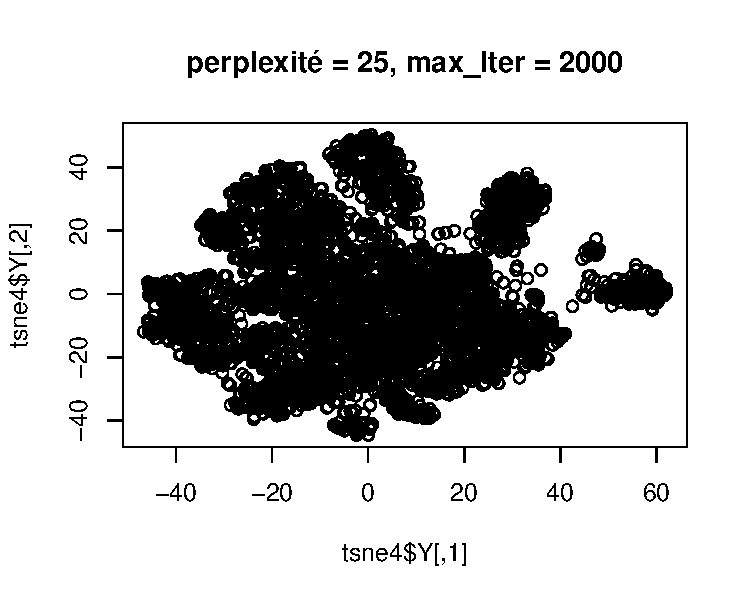
\includegraphics{Analyse_Exploratoire_Projet_files/figure-latex/unnamed-chunk-20-4} \end{flushleft}

\begin{flushleft}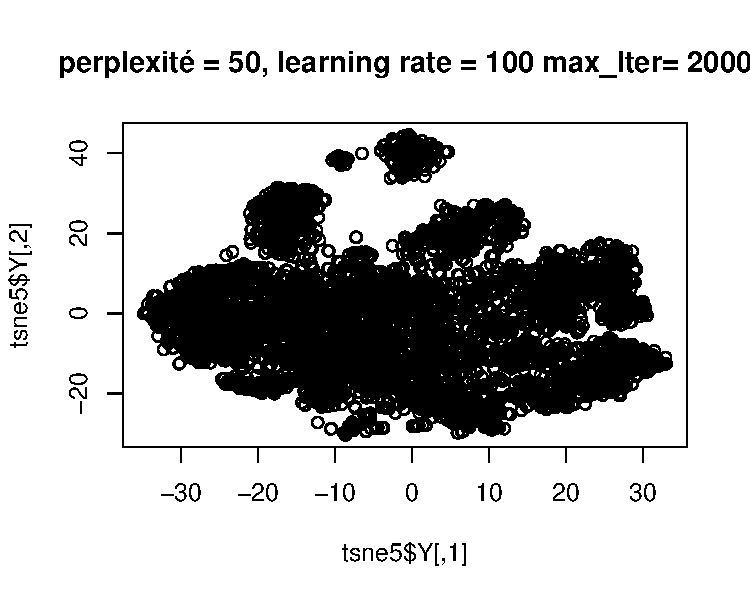
\includegraphics{Analyse_Exploratoire_Projet_files/figure-latex/unnamed-chunk-20-5} \end{flushleft}

\begin{flushleft}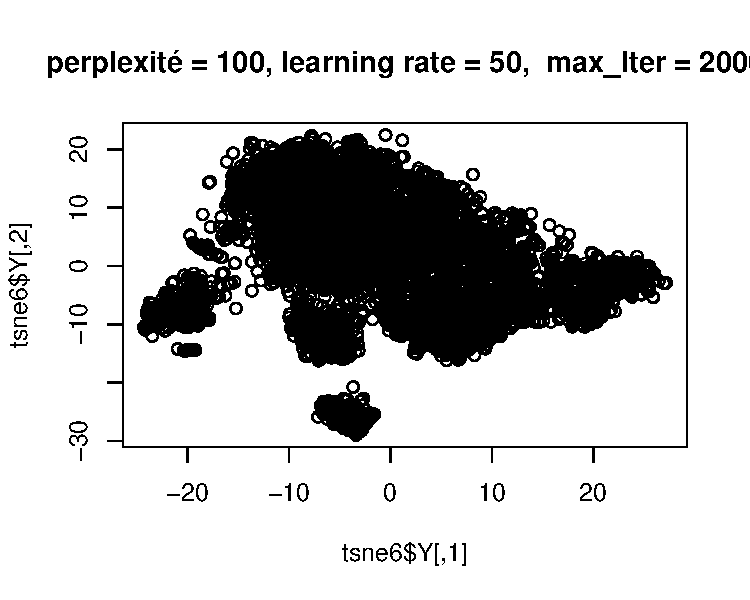
\includegraphics{Analyse_Exploratoire_Projet_files/figure-latex/unnamed-chunk-20-6} \end{flushleft}

~

Les graphiques montrent une ségmentation qui devient plus nette en augmentatnt la perplexité et en diminuant le pas d'apprentissage.

~

Nous pouvons affecter un numéro à chaque segment, et enrichir le dataset d'une nouvelle colonne spécifiant le cluster de chaque observation:

~

\begin{verbatim}
# Utiliser l'algorithme kmeans pour départager les observations entre groupes ( choix graphiquement orienté de 4 groupes)

kmeans.result = kmeans(tsne6$Y, centers=4)

colonne.groupe = as.data.frame(kmeans.result$cluster)

colnames(colonne.groupe) = "Groupe"

data.groupe = cbind(d, colonne.groupe)

table(data.groupe$Groupe)
\end{verbatim}

\begin{verbatim}
## 
##    1    2    3    4 
## 1500 1284  958 1258
\end{verbatim}

~

\hypertarget{analyse-des-donnuxe9es-catuxe9gorielles}{%
\section{Analyse des données catégorielles}\label{analyse-des-donnuxe9es-catuxe9gorielles}}

Dans la suite nous nous intérressons aux données catégorielles. L'échantillon représentatif des données est enrichie de la colonne ``Groupe'' récupérée précédemment. Notre dataframe est désormais composé de 5000 observations et de 22 variables catégorielles.

~

\begin{verbatim}
##       new_cell crclscod asl_flag prizm_social_one                area dualband
## 51663        Y       BA        N                C        HOUSTON AREA        Y
## 57870        U       AA        N                C ATLANTIC SOUTH AREA        Y
## 2986         Y        A        N                U        HOUSTON AREA        Y
## 29925        U       BA        N         inconnue        CHICAGO AREA        Y
## 95246        Y       BA        N                U  NEW YORK CITY AREA        Y
## 68293        U       ZA        Y                S        CHICAGO AREA        Y
##       refurb_new  ownrent dwlltype marital infobase HHstatin dwllsize ethnic
## 51663          R inconnue inconnue       U inconnue inconnue inconnue      O
## 57870          N        O        S       S        M        C        A      S
## 2986           N        O        S       M        M        C        A      N
## 29925          N        O        S       U        M        C        A      N
## 95246          N        O        M       U        M inconnue        C      H
## 68293          R        O        S       S        M        H        A      H
##       kid0_2 kid3_5 kid6_10 kid11_15 kid16_17 creditcd churn Groupe
## 51663      U      U       U        U        U        N     1      1
## 57870      U      U       U        U        U        Y     0      3
## 2986       U      U       U        Y        U        Y     1      2
## 29925      U      U       U        U        U        Y     1      1
## 95246      U      U       U        U        U        Y     1      2
## 68293      U      U       U        U        U        N     0      4
\end{verbatim}

~

\hypertarget{afc-entre-churn-et-new_cell}{%
\subsection{AFC entre ``churn'' et ``new\_cell'':}\label{afc-entre-churn-et-new_cell}}

~

La variable \textbf{churn} prend les valeurs 1 et o, respectivement pour l'état 1 d'avoir résilié dans les deux mois suivant l'observation, et l'état 0 d'être toujours abonné sur le même intervalle de temps.

~

La variable \textbf{new\_cell} quant à elle, indique si'utilisateur dispose d'un nouveau téléphone avec les initiales de ``Yes'', ``No'' et ``Unknown''.

~

Après Construction du tableau de contingence entre les deux variable, la répartition des modalités est visible sur la figure suivante:

~

\begin{flushleft}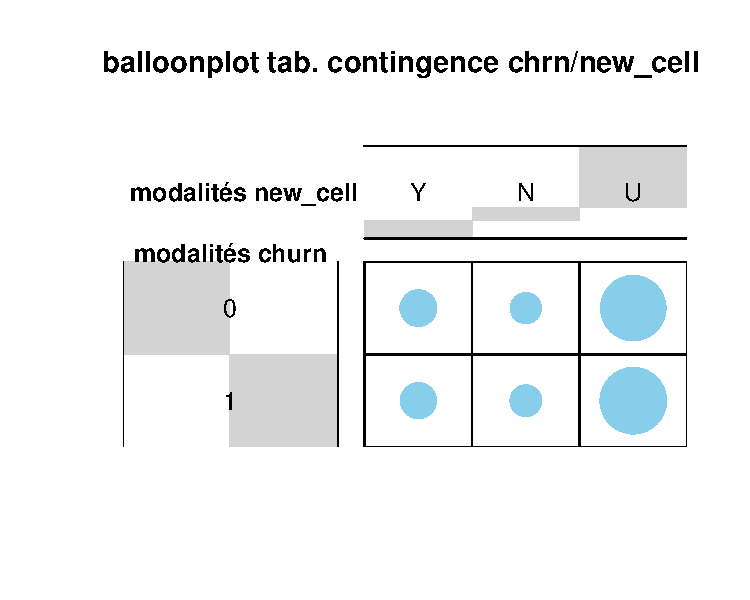
\includegraphics{Analyse_Exploratoire_Projet_files/figure-latex/unnamed-chunk-23-1} \end{flushleft}

~

Cette figure nous donne une indication visuelle : les individus ayant une modalité de la variable \textbf{new\_cell} semblent être répartis de façon égale sur les deux modalités de la variable \textbf{churn}.

~

L'hypothèse H0 que les deux variables soient indépendantes peut être formulée. Un Test du chi squared avec cette hypothèse est réalisé:

~

\begin{verbatim}
## 
##  Pearson's Chi-squared test
## 
## data:  contingence1
## X-squared = 0.95079, df = 2, p-value = 0.6216
\end{verbatim}

~

La p\_value de ce test est de 0.62, l'hypothèse H0 ne peut être rejetée dans ces conditions. Nous ne pouvons rejeter l'hypothèse de l'indépendance de ces deux variables.

~

Les variables \textbf{churn} et \textbf{new\_cell} peuvent être considérée comme indépendantes (avec un risque beta de second espèce de nous tromper).

~

\hypertarget{afc-entre-ownrent-et-ethnic}{%
\subsection{AFC entre ``ownrent'' et ``ethnic'':}\label{afc-entre-ownrent-et-ethnic}}

~

(Il est à préciser qu'avant de se tourner vers ce couple facile, plusieurs autres combinaisons de variables plus utiles ont été testées et se sont malheureusement montrées pas concluantes. En particulier la paire Group-churn dont l'indépencance n'a pu être rejetée par le chisq test, et la paire churn-ethnic qui était bel et bien dépendante mais qui posait un problème de dimension lors du plottage).

~

La variable \textbf{ownrent} prend les valeurs ``O'',``R'' et ``inconnue'', respectivement pour l'état de ``propriétaire'', ``locataire'' ou ``situation inconnue''.

~

La variable \textbf{ethnic} quant à elle, permet d'attribuer un groupe éthnique au client, représenté par 17 lettres. Trois modalités de cette variable sont exclues car trop rare. Une modalité supplémentaire est la valeur ``inconnue''.

~

Après Construction du tableau de contingence entre les deux variable, la répartition des modalités est visible sur la figure suivante:

~

\begin{flushleft}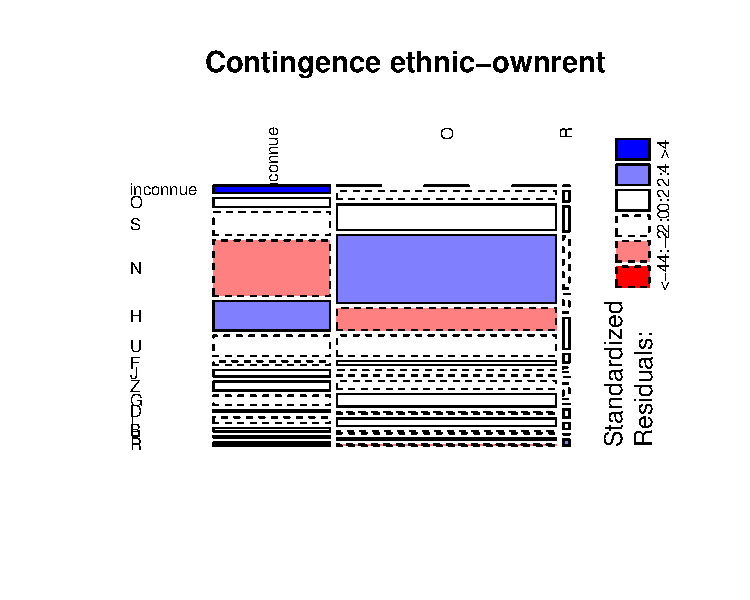
\includegraphics{Analyse_Exploratoire_Projet_files/figure-latex/unnamed-chunk-25-1} \end{flushleft}

~

la distribution des modalités des deux variables semble indiquer une corrélation. Appliquons le test du chisq avec l'hypothèse H0 que le les deux variables soient indépendantes:

~

\begin{verbatim}
## 
##  Pearson's Chi-squared test
## 
## data:  contingence2
## X-squared = 193.39, df = 28, p-value < 2.2e-16
\end{verbatim}

~

L'hypothèse d'indépendance des variables \textbf{churn} et \textbf{ethnic} est rejeté avec une p\_value extrêmement faible de 2.2e-16.

~

Ces deux variables peuvent être considérées comme dépendantes avec un risque quasi nul de nous tromper.

~

Après avoir appliqué une analyse factorielle des correspondances, visualisons l'inertie des valeurs propres:

~

\begin{flushleft}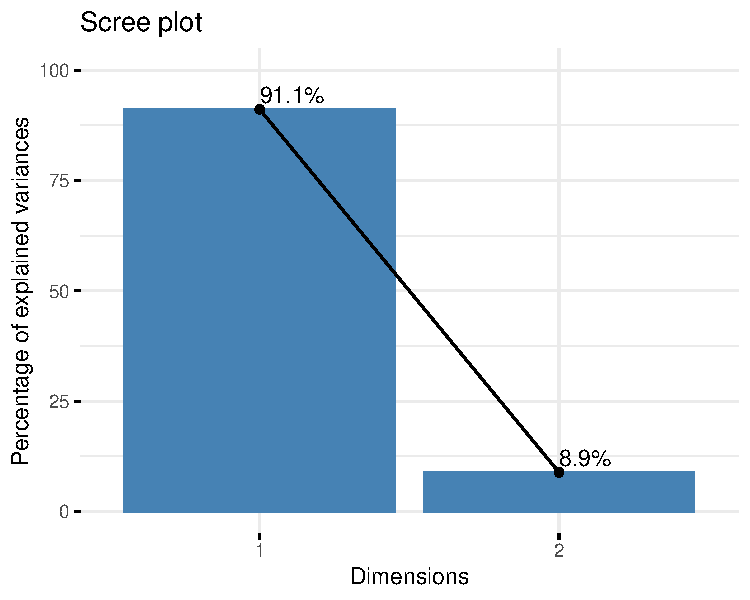
\includegraphics{Analyse_Exploratoire_Projet_files/figure-latex/unnamed-chunk-27-1} \end{flushleft}

~

Les 2 premiers axes de l' analyse expriment \textbf{100\%} de l'inertie totale du jeu de données ; cela signifie que 100\% de la variabilité totale du nuage des lignes (ou des colonnes) est représentée dans ce plan. ( Ce résultat était prévisible car max(valeurs propres) = min((p-1), (n-1)))

~

Le premier axe factoriel est largement prépondérant : il explique a lui seul 91.14\% de la variance totale des données.

~

La variance expliquée par le premier axe peut suffire pour le choisir comme unique axe dans la réduction de dimension, nous choisirons néanmoins de garder graphiquement le deuxième axe pour des raisons de visibilité.

~

Visualisation de profils lignes:

\begin{flushleft}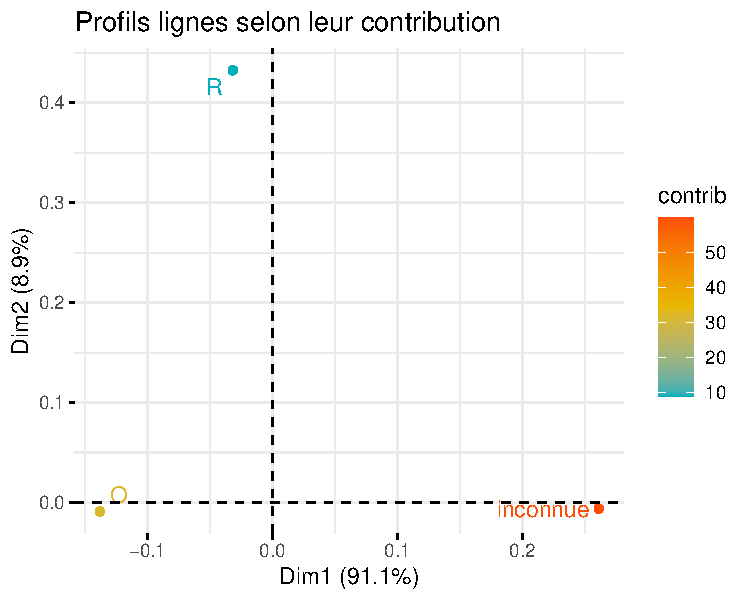
\includegraphics{Analyse_Exploratoire_Projet_files/figure-latex/unnamed-chunk-28-1} \end{flushleft}

~

Le profil des ``O'' ( propriétaire de logement) caractérise le côté négatif du premier axe factoriel, par opposition au profil des ``inconnue'' (état inconnu de la proprieté) qui caractérise le côté positif du premier axe factoriel.

~

Le profil des ``R'' ( locataires) est bien projeté sur le deuxième axe mais avec une faible contribution.

~

Les profils ``O'' et ``inconnue'' ne partageront pas le même type type de modalités ``ethnic''

~

Visualisation de profils colonnes:

~

\begin{flushleft}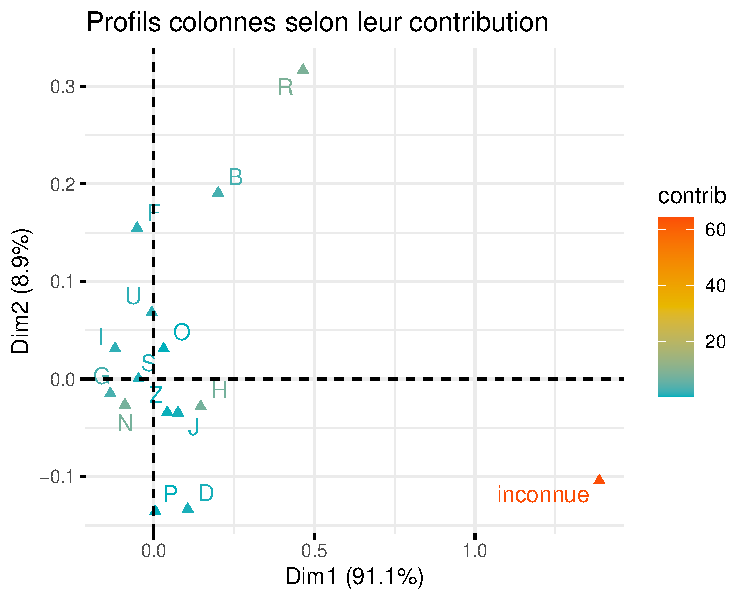
\includegraphics{Analyse_Exploratoire_Projet_files/figure-latex/unnamed-chunk-29-1} \end{flushleft}

~

Le profil des ``inconnue'' ( pas d'étiquette éthnique ) caractérise le côté positif du premier axe factoriel.

~

Projection simultanée des profils lignes et profils colonnes:

~

\begin{flushleft}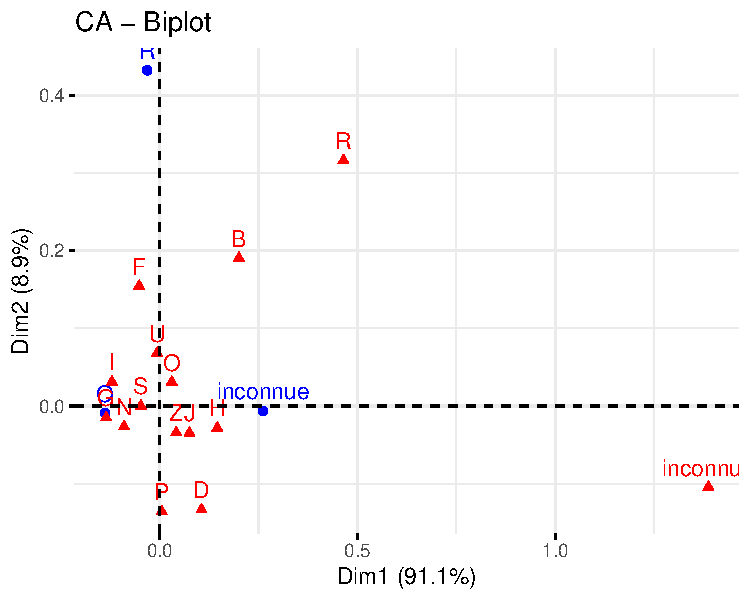
\includegraphics{Analyse_Exploratoire_Projet_files/figure-latex/unnamed-chunk-30-1} \end{flushleft}

~

\hypertarget{analyse-des-correspondances-multiples}{%
\subsection{Analyse des correspondances multiples:}\label{analyse-des-correspondances-multiples}}

Dans la suite, une analyse des correspondances multiples est appliquée aux variables :

~

`new\_cell', `crclscod', `asl\_flag', `prizm\_social\_one', `area', `dualband', `refurb\_new', `ownrent', `dwlltype', `marital', `infobase', `HHstatin', `dwllsize', `ethnic', `kid0\_2', `kid3\_5', `kid6\_10', `kid11\_15', `kid16\_17', `creditcd'

soient toutes les variables catégorielles, sauf ``churn'' et ``Group''.

~

Suite à l'analyse, la figure suivante permet de visualiser les valeurs propres calculées pour chaque axe factoriel:

~

\begin{flushleft}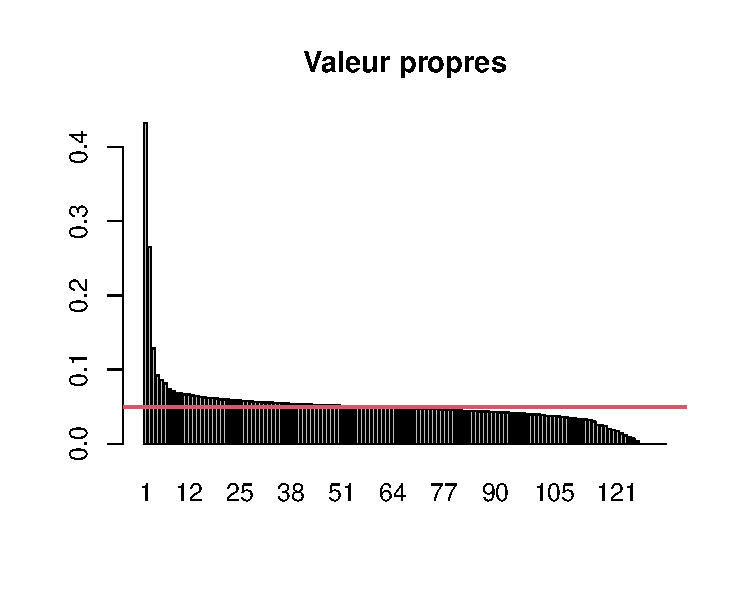
\includegraphics{Analyse_Exploratoire_Projet_files/figure-latex/unnamed-chunk-31-1} \end{flushleft}

\begin{verbatim}
## [1] 133   3
\end{verbatim}

~

La ligne rouge y=0.05 représente la moyenne des valeurs propres ( 1/s).

~

Les valeurs propres sont très nombreuses, au nombre de 133 ( p - s ).

~

Ce résultat n'est pas satisfaisant car il ne permet pas d'isoler des valeurs propres significatives.

~

Nous procédons à une correction de Benzécri afin de limiter les biais dus à la fréquence des modalités.

~

La figure suivante permet de visualiser les valeurs propres après correction:

~

\begin{flushleft}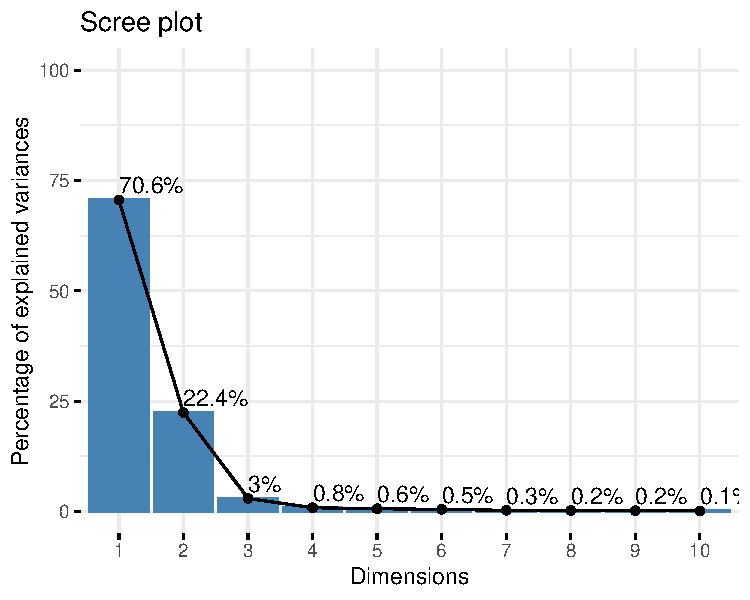
\includegraphics{Analyse_Exploratoire_Projet_files/figure-latex/unnamed-chunk-32-1} \end{flushleft}

~

Cette correction était bel et bien fructive, puisqu'elle nous permet désormais d'isoler les deux premiers axes factoriels, qui captent à eux seuls 93\% de la variance.

~

Le résultat de cette correction sera utilisé dans la suite pour la construction des graphes et la détermination des contributions des modalités et individus dans la construction des axes.

~

\textbf{Analysons le résultat des modalités:}

~

\begin{flushleft}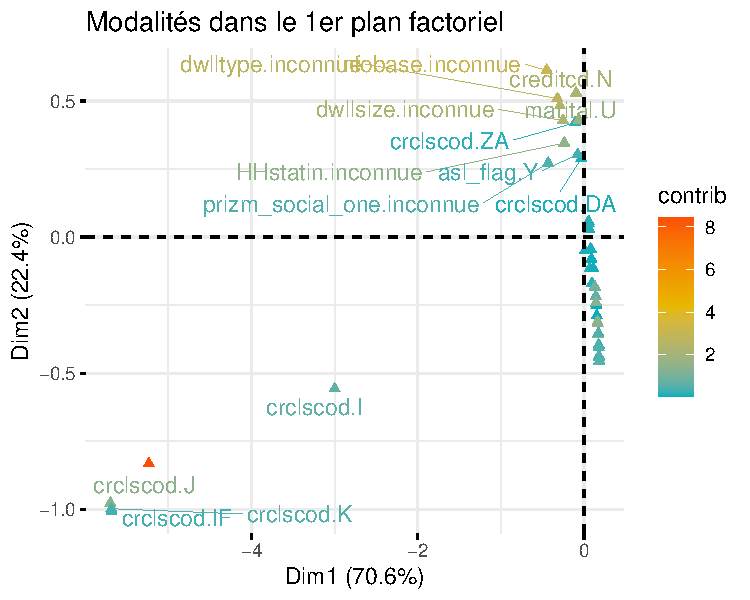
\includegraphics{Analyse_Exploratoire_Projet_files/figure-latex/unnamed-chunk-33-1} \end{flushleft}

~

\textbf{AXE 1 :}

~

Le côté négatif de la première dimension est caractérisé par clients ayant les modalités : ``marital.inconnue'', ``ethnic.inconnue'', ``kid0\_2.inconnue'', ``kid3\_5.inconnue'', ``kid6\_10.inconnue'', ``kid11\_15.inconnue'', ``kid16\_17.inconnue'', ``creditcd.inconnue'' et ``crclscod.J''.

~

L'analyse des cos2 et contributions ne permet pas de déterminer de façon significative des modalités caractérisant le côté positif du premier axe factoriel.

~

\textbf{AXE 2 :}

~

Le côté négatif de l'axe 2 est caractérisé par des clients ayant les modalités: ``dwllsize.A'', ``dwlltype.S'', ``ownrent.O'', ``marital.M'' et ``creditcd.Y''.

~

Le côté positif de l'axe 2 est caractérisé par des clients ayant les modalités: ``creditcd.N'', ``infobase.inconnue'', ``ownrent.inconnue'', ``dwllsize.inconnue'', ``dwlltype.inconnue'' et ``marital.U''.

~

\textbf{Analysons le résultat des Individus:}

~

\begin{flushleft}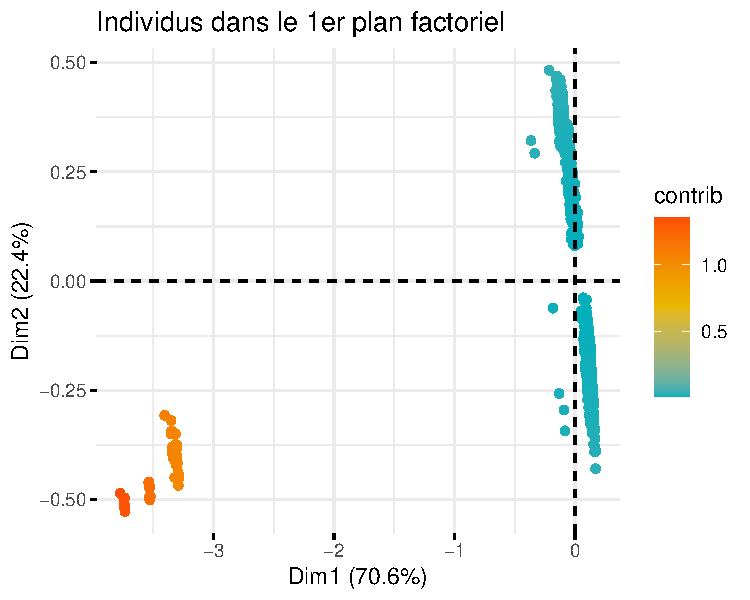
\includegraphics{Analyse_Exploratoire_Projet_files/figure-latex/unnamed-chunk-34-1} \end{flushleft}

~

\textbf{AXE 1 :}

~

Le côté négatif de la première dimension est caractérisé par les individus : 42611, 31911, 43650, 40744, 45566, 58263, 36345, 30455, 67719, 55247, 41538, 35533, 46415, 32463, 40160, 45711.

~

L'analyse des cos2 et contributions ne permet pas de déterminer de façon significative des individus caractérisant le côté positif du premier axe factoriel.

~

\textbf{AXE 2 :}

~

Le côté positif de l'axe 2 est caractérisé par les individus: 91895, 56753, 93970, 54525, 78186, 96084.

~

Le critère conjoint du cos2 et de la contribution ne permettent pas d'identifier de façon indiscutable des individus caractérisant le côté négatif du deuxième axe factoriel.

~

**Projection simultanée des individus et modalités:

~

\begin{flushleft}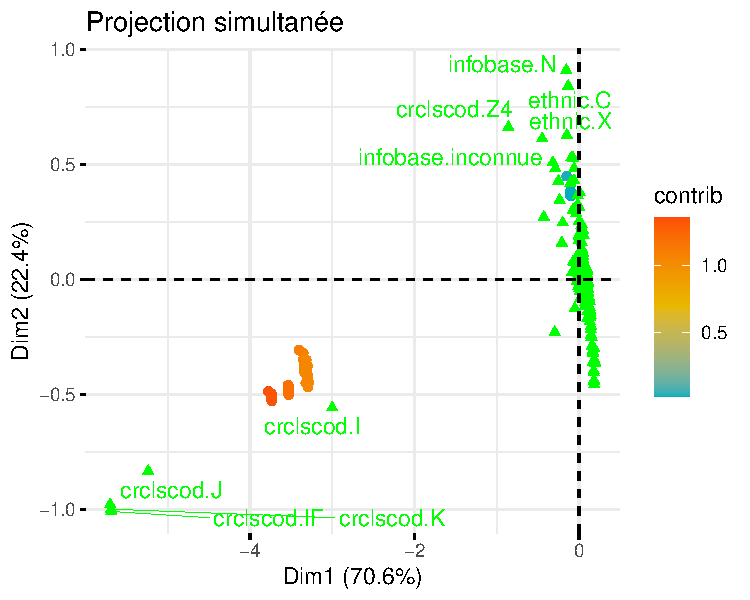
\includegraphics{Analyse_Exploratoire_Projet_files/figure-latex/unnamed-chunk-35-1} \end{flushleft}

~

\hypertarget{conclusion}{%
\section{Conclusion:}\label{conclusion}}

~

Nous disposons d'un set de données de qualité. dans cette entreprise, un soin a été apporté à collecter un nombre élevé de caractéristiques chez le client, avec une quantité de valeurs manquantes qui reste relativement faible par rapport à la taille totale du jeu et les normes en vigueur.

~

Le travail sur un jeu de données aussi important, cent milles observations sur cent variables différentes, soient dix millions de cases remplies, rencontre des limites techniques de mémoire et de rapidité de calcul sur un matériel grand public. Et nécéssite par conséquent de faire appel à une méthode fiable de réduction du volume d'observations à traiter, dans notre cas un échantillonnage aléatoire réduisant par vingt le nombre de lignes retenues pour l'analyse.

~

Réaliser un modèle prédictif, pour anticiper certains comportements du client ( exemple : résiliation d'un abonnement),est l'un des enjeux de l'analyse de ces données. Néanmoins, modéliser avec toutes les variables nuit à la qualité du modèle. D'une part en augmentant le coût de la requête en ressources. D'autre part en diminuant la lisibilité de l'information extraite. La \textbf{PCA} nous aide à remédier à ce désagrément en réduisant drastiquement le nombre de dimensions à considérer, grâce à la synthèse de peu de composantes principales non corrélées à partir d'un grand nombre de variables corrélées. Dans notre cas, l'analyse en composantes principales de nos données quantitatives a permis de dégager un premier plan factoriel captant 44.3 \% de la variance. Dans ce premier plan factoriel, le premier axe est positivement caractérisé par neuf variables très corrélées, qui sont des moyennes du nombre d'appels ou des durées d'appel sur différents intervalles de temps. Le deuxième axe est quand à lui positivement caractérisé par le nombre d'accès au service internet de l'abonnement.

~

Essayer de dégager des profils type chez les clients est également un enjeu majeur pour l'entreprise. Segmenter les clients en fonction de leurs modes de consommation permet de cibler les offres commerciales entre autres, ce qui permet de limiter le coût d'une campagne tout en gagnant en efficacité. L'algorithme \textbf{T-SNE} a été appliqué aux données quantitatives, afin de déceler une proximité entre individus dans un espace réduit. Différents essais avec des réglages différents des hyper-paramètres, montrent un tropisme des observations à s'agglutiner en petit îlots. En particulier, un réglage avec un petit pas d'apprentissage et une grande valeur de la perplexity et du maximum d'itérations, permet de visualiser graphiquement, dans un espace à deux dimensions, la différenciation des coordonnées des individus en 4 clusters au moins. L'application de l'algorithme \textbf{Kmeans} a permis ensuite d'affecter un numéro de groupe à chaque cluster. Cette donnée est ajoutée au set d'analyse sous forme d'une nouvelle colonne appelée ``Group''. Deux individus appartenant au même groupe sont censés partager des caractéristiques communes, reflétant un comportement ou des préférences similaires.

~

L'analyse des données qualitatives, a permis initialement de s'apercevoir que le fait de posséder un nouveau terminal n'influençait pas le fait de se désabonner chez un client.

~

Une analyse factorielle des correspondances (\textbf{AFC}) a été initiée avec la nouvelle variable ``Group'' et la variable ``churn''. l'hypothèse de l'indépendance de ces deux variables n'a pu être rejetée avec un seuil de significativité de 5\%. Elle aurait pu l'être avec un seuil de 6\% mais le choix a été fait d'avorter l'analyse. Ce manque de significativité dans le lien entre ces deux variables pourrait être interpreté par le fait que tous les groupes se comportent de façon identique par rapport au désabonnement (le churn). Mais il est plus probable, qu'un set de données plus nettoyé (exemple: supprimer les valeurs''inconnue''), et un meilleur affinage des hyper-paramètres avec \textbf{T-SNE}, nous auraient permis de segmenter de façon plus juste les individus, et nous auraient ainsi permis de rejeter fermement l'hypothèse de l'indépendance entre ces deux variables.

~

L'analyse des correspondances multiples (\textbf{ACM}) a permis quant à elle de dégager un premier plan factoriel captant à lui seul 93 \% de la variance, avec un premier axe prépondérant ayant capté plus de 70 \% de la variance. Les modalités ``inconnue'' de 9 variables caractérisent négativement le premier axe. Cette valeur ``inconnue'' est une valeur qui a été recodée en remplacement d'une chaine vide en phase de prétraitement, car l'hypothèse de travail initiale était que les vraies valeurs manquantes (missing values) avaient pour valeur n.a. Il peut être judicieux de changer d'hypothèse de travail et de considérer la valeur ``inconnue'' comme faisant partie de la data manquante, et de lui appliquer les prétraitements nécéssaires pour une nouvelle analyse.

~

Ces différentes analyses ont été l'occasion de confronter des difficultés pratiques et de se familiariser avec un jeu de données riche. Ce dernier se prête à différentes autres formes d'analyse. La suite envisagée pour cet agréable travail, est de le réaffiner et de l'enrichir, en mettant en application des techniques de \textbf{modélisation linéaire}.

~

\hypertarget{references}{%
\section*{References}\label{references}}
\addcontentsline{toc}{section}{References}

\citet{Analyse}, \citet*{Extraction}

\begin{supplement}
\stitle{Annexe 1, liste complète des variables}
\sdescription{}
\end{supplement}

\begin{acks}[Acknowledgments]
Toute ma gratitude à mes professeurs pour tout le savoir qu'ils nous ont transmis.Une pensée optimiste à ceux qui défendent nos droits.
\end{acks}

\bibliographystyle{ba}
\bibliography{sample.bib}


\end{document}
